\begin{figure}[!htbp]
\centering
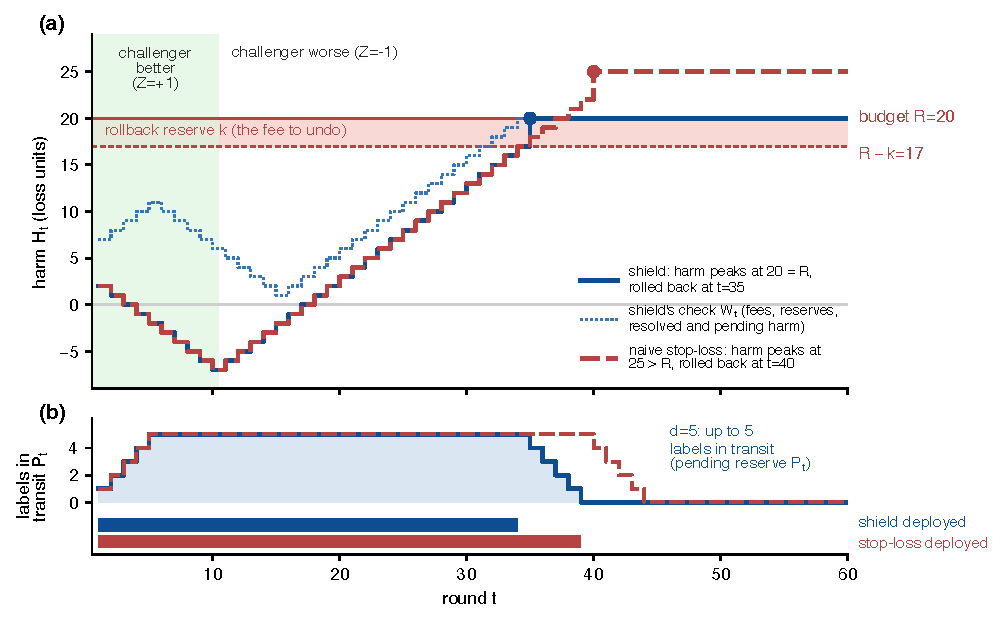
\includegraphics[width=\linewidth]{figures/fig_mechanism_full.pdf}
\caption{Full detail for the tape of Figure~\ref{fig:mechanism}. (a) Realised harm $H_t$ of the shield (solid) and of the stop-loss (dashed), with the shield's check (dotted: fees, rollback reserve $k$, resolved and pending harm; see $W_t$ in Section~\ref{sec:method}). The check is evaluated before the query coin and action; values are plotted at round $t$ after charging its exposure. The shaded band lies between $R-k$ and $R$. (b) Labels in transit and rounds on which each controller is deployed.}
\label{fig:mechanism_full}
\end{figure}
